\section{Vibration Acquisition Channel}\label{sec:vibration-acquisition-channel}

\subsection{Accelerometer}\label{ssec:accelerometer-signal}
	The choosen accelerometer for this project was the \textit{ADXL335} from \textit{Analog Devices} \cite{devices2010adxl335}. This accelerometer was choosen because it is the cheapest one availabe with the following characteristics:

	\begin{itemize}
		\item It has 3 axis sensing (easy to install).
		\item Low power operation (350$\mu$A).
		\item 10,000 g shock survival.
		\item 1V8-3V3 Single-supply operation.
		\item $\pm$3g measurements.
	\end{itemize}

	When powered up with 3V3 the sensor has a linear voltage output of 0V for -3g and 3V3 for 3g. This sensor is ideal for this project, the only issue is the installation. The sensor comes in a 16-LFCSP IC (Figure \ref{fig:16lfcsp}), and this IC needs to be installed where acceleration is intended to be measured, so a additional board is necessary to install it. 

	\begin{figure}[htbp]
		\centering
		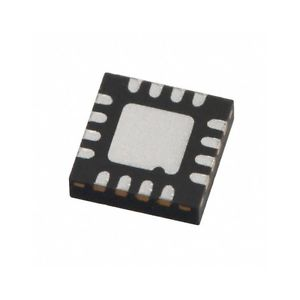
\includegraphics[width=.8\textwidth]{figuras/fig-16lfcsp.jpg}
		\caption{16-LFCSP \cite{16lfcsp}}
		\label{fig:16lfcsp}
	\end{figure}

	The are already embdded solutions that can solve this issue, such as the \textit{Adafruit ADXL335 - 5V ready} \cite{adafruit-5v-ready}. This small (19mm x 19mm) board (Figure \ref{fig:adafruit-adxl335}) has the ADXL335 with the capacitors recommended by the datasheet, with a 3V3 voltage regulator so the board can be powererd up with 5V and with the mounting holes to fix the board in any surface, making it ideal for this project.

	\begin{figure}[htbp]
		\centering
		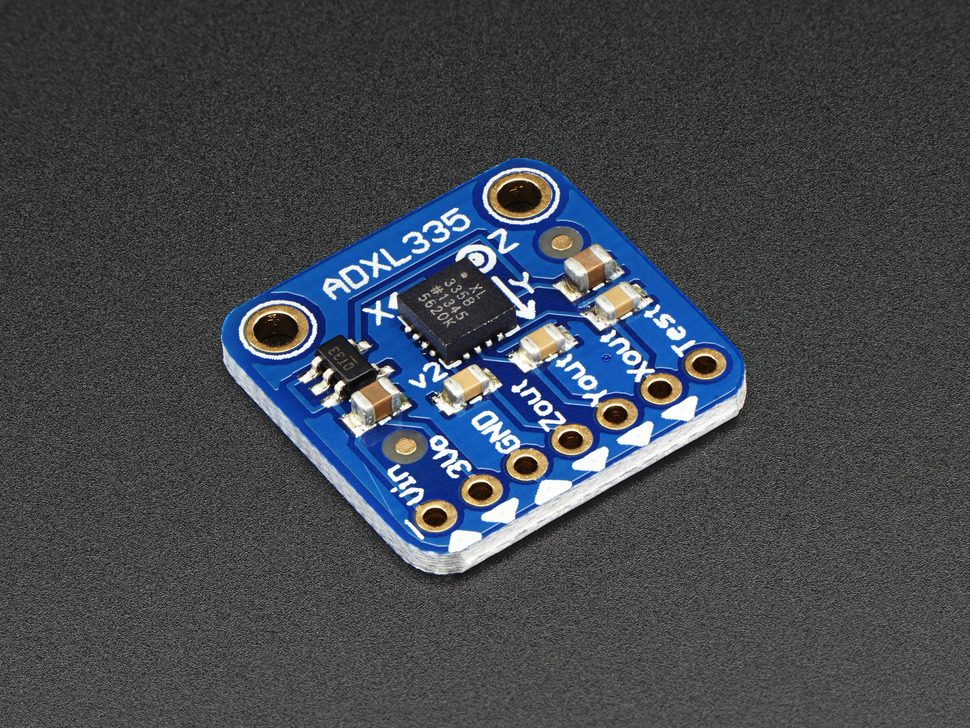
\includegraphics[width=.8\textwidth]{figuras/fig-adafruit-adxl335.jpg}
		\caption{Adafruit ADXL335 - 5V ready \cite{adafruit-adxl335}}
		\label{fig:adafruit-adxl335}
	\end{figure}


\subsection{Signal Conditioning Circuit}\label{ssec:accelerometer-signal-conditioning-circuit}

	The ADXL335 datasheet \cite{devices2010adxl335} says that for a -3g measured acceleration the device output is of 0V and for +3g measurement it is 3V3 voltage. The sensor conditioning circuit is displayed on Figure \ref{fig:accelerometer-signal-conditioning-circuit}.

	\begin{figure}[htbp]
		\centering
		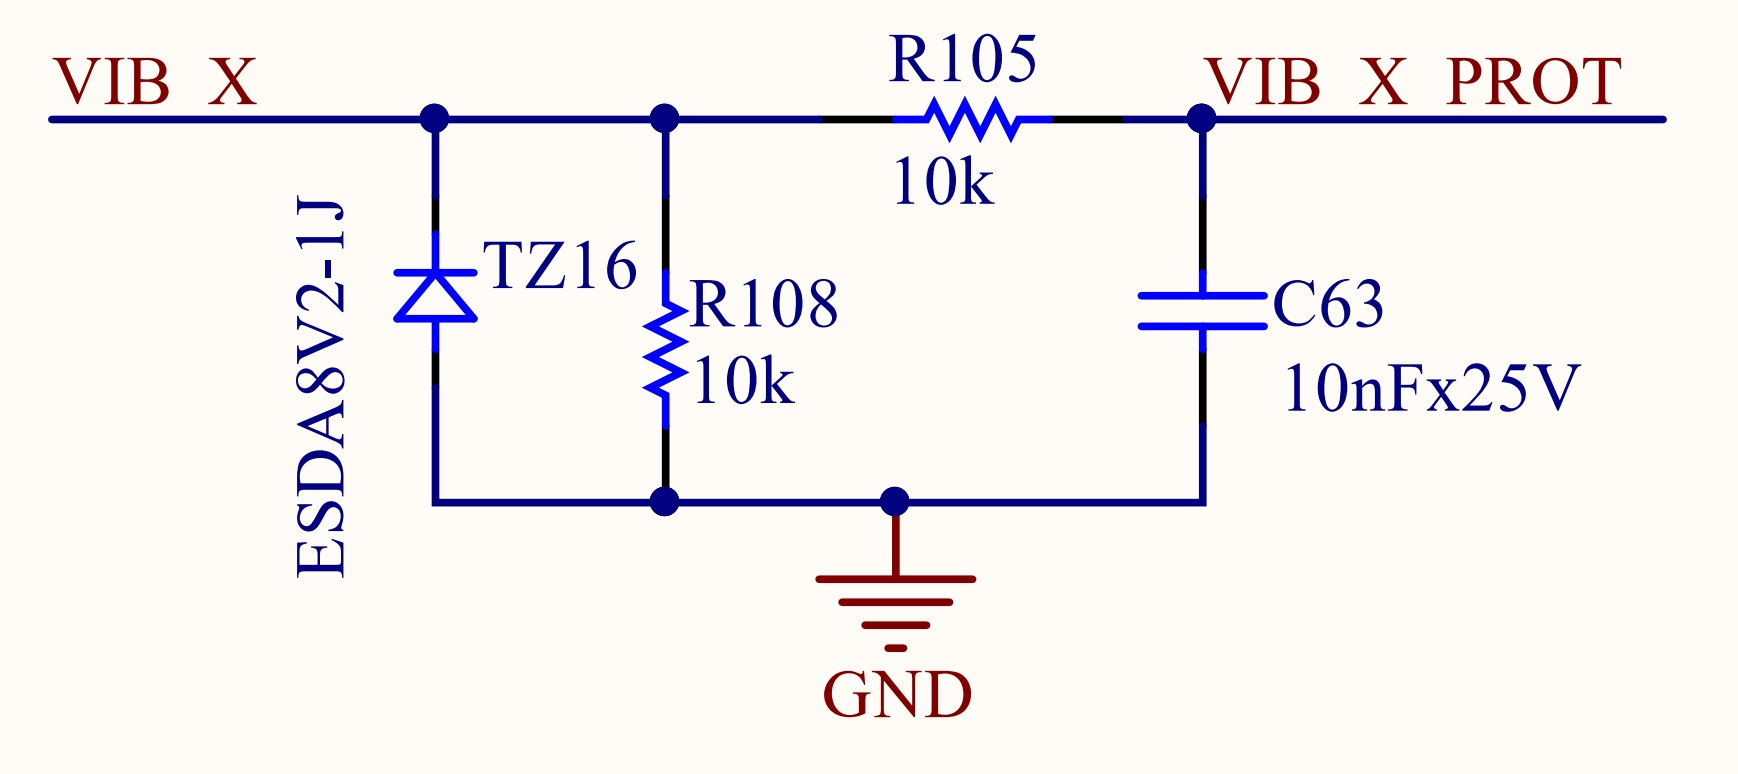
\includegraphics[width=.8\textwidth]{figuras/fig-accelerometer-signal-conditioning-circuit}
		\caption{Accelerometer Signal Conditioning Circuit}
		\label{fig:accelerometer-signal-conditioning-circuit}
	\end{figure}


	The circuit is composed only of a protection and filtering circuit. TZ16 is a TVS with a standoff reverse voltage of 5V, R105 and C63 form a LPF with cutoff frequency of aproximately 1.6kHz, which should not intervene with the passband signal.

\subsection{Sensor Detection Circuit}\label{ssec:accelerometer-sensor-detection-circuit}

	The choosen solution for the accelerometer \textit{(Adafruit ADXL335 - 5V ready)} has a integrated 3V3 voltage regulator. In Figure \ref{fig:adafruit-adxl335} it is possible to see that the 3V3 voltage output from the voltage regulator has a connection point on the board. Hence, if a wire is connected to this point and to the main circuit board, whenever this point does not have 3V3 voltage the sensor is disconnected. Moreover, the detection circuit just need to detect when the net is in 0V or 3V3.
	\par
	The detection circuit can be seen in Figure \ref{fig:accelerometer-sensor-detection-circuit}, D14 is a schottky diode used to protect the input from polarity change. TZ19 is a TVS used to protect the circuit from overvoltage, R111 and C66 forms a LPF with cutoff frequency close to 16Hz used to protect the NMOS gate from any fast transient.s

	\begin{figure}[htbp]
		\centering
		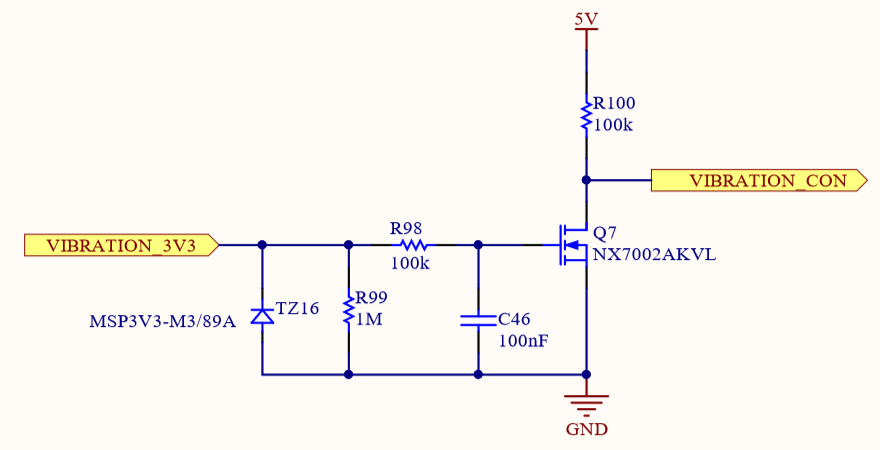
\includegraphics[width=.8\textwidth]{figuras/fig-accelerometer-sensor-detection-circuit.png}
		\caption{Accelerometer Sensor Detection Circuit}
		\label{fig:accelerometer-sensor-detection-circuit}
	\end{figure}